\chapter{Regularization of Loss Functions}
\label{ch-regularization}

\begin{figure}[h!]
\centering
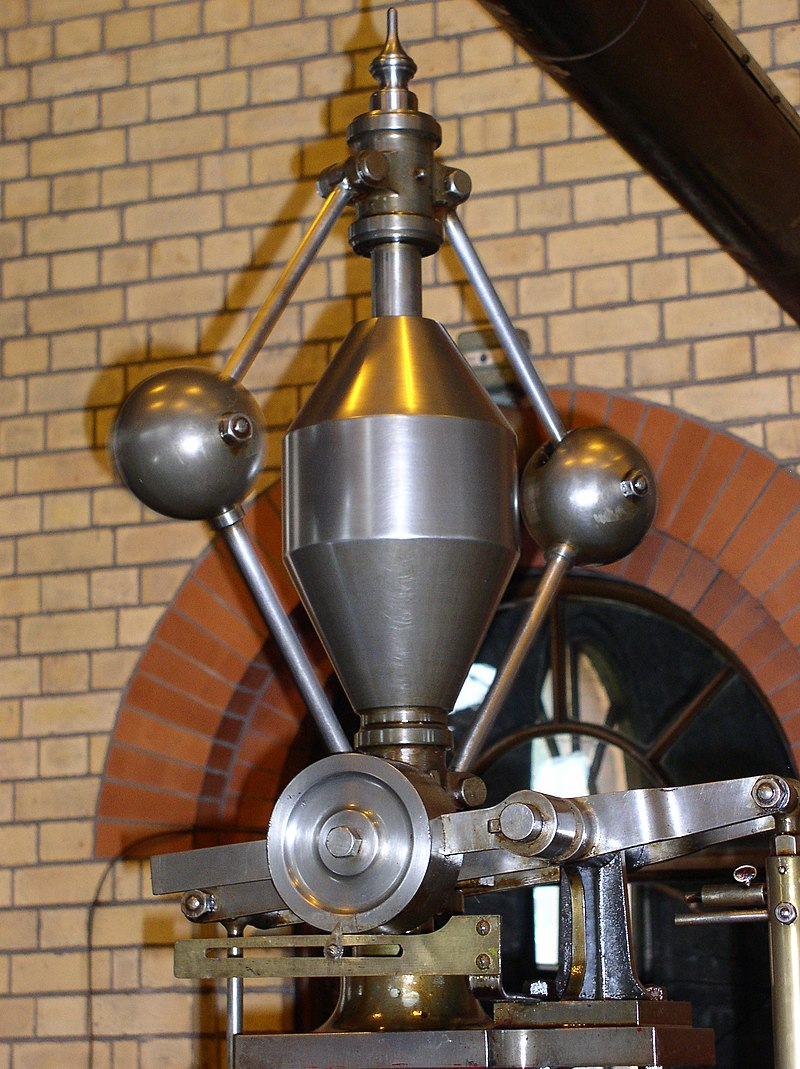
\includegraphics[height=3in]
{regularization/steam-guv.png}
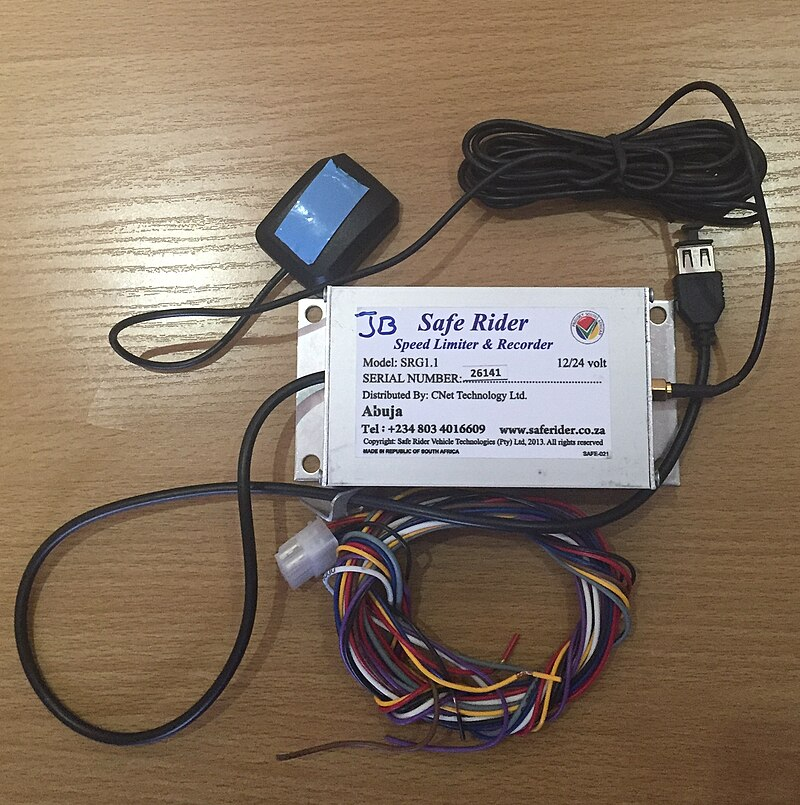
\includegraphics[height=3in]
{regularization/electronic-guv.png}
\caption{Flyball governor for a steam engine, and an electronic governor for an electrical motor.}
\label{fig-guv-device}
\end{figure}

Whenever I hear the words \qt{regulator} or \qt{regularization}, the first 
thing I think of is a
{\bf governor} (a.k.a. regulator, controller, speed limiter, flyball governor). (See Fig.\ref{fig-guv-device} and Wikipedia Ref.\cite{wiki-guv-device})
A governor is a feedback device that regulates the speed at which 
a machine spins, preventing it from spinning faster than a certain threshold. It was originally invented by Christiaan Huygens for windmills and later adapted by James Watts for steam engines. This chapter is about a mathematical construct whose purpose is analogous to that of the mechanical governor.




 The topic
 of this chapter is Regularization of Loss functions (ROLF).

ROLF is the practice of adding
a convex function  $\calr:\RR^n\rarrow \RR$
(called the {\bf regulator function}\footnote{This function is also commonly called a {\bf penalty function}.
It can  also be thought  of, from a Bayesian perspective,
as the log of a prior probability, and the loss function can be thought of as a log likelihood function.}) to
a convex function  $\call:\RR^n\rarrow \RR$
(called the {\bf  loss function}\footnote{This function is also commonly
called the {\bf cost or error function}.}), when one
wishes to minimize the loss function. In Machine Learning,
the variable being minimized over is often the weights
of a Neural Net, so we will denote it by $w\in \RR^n$, and use $w^*\in \RR^n$
to represent the
minimum of $\call^+(w) =\call(w)+ \calr(w)$.

In some cases (like in $L^p$ norm ROLF,
which we discuss below),
the minimum of $\call^+(w)$
and that of $\call(w)$
are not the same but very close. In such cases,
displacing the minimum of
$\call(w)$
might be done in order
to avoid overfitting, or
to spread out degenerate solutions, or to produce
sparse solutions.

In other cases (like in proximal ROLF, which we discuss below),
the minimum of $\call^+(w)$
and that of $\call(w)$
are the  same.
In such cases, ROLF might be done
to improve the
convergence properties
of a sequence of points
$\{w_k\}_{k=0}^\infty$
such that $w_k\rarrow w^*$
as $k
\rarrow \infty$.

There are many methods
of biasing the
minimum of a convex function that  don't
involve adding a regulator
function.
For example, Early Stopping
of training
and Cross Validation for Neural Nets,
or adding Latent Variables
to a Bayesian Network.
Or Constraint Optimization where hard equality and/or inequality constraints are imposed (as in Linear Programming,
Lagrange multipliers, Khun-Tucker conditions, method of simple substitution of constraints).
We won't discuss those types of
ROLFs in this chapter\footnote{ROLF that adds a regulator function (resp., doesn't add)
is sometimes called {\bf Explicit (resp., Implicit)
regularization}.}, except for a brief section on latent nodes at the end.



Loss functions commonly used in Statistics and
Machine Learning (ML) are of the form


\beq
\call(w) = \sum_{\s=1}^{nsam}
\HAT{\call}(\haty_\s(x_\s, w), y_\s)
\eeq
where the sum is over $nsam$ samples.
A common, more specific type of $\call(w)$ is the
{\bf mean square error} which is
given by


\beq
\call(w) = \frac{1}{nsam}\sum_{\s=1}^{nsam}
\norm{\haty_\s(x_\s, w)-y_\s)}_2
\eeq
This loss function is convex, so it has a minimum:

\beq
\left\{
\begin{array}{l}
w^* = \argmin_w \call(w)
\\
Loss = \min_w \call(w) = \call(w^*)
\end{array}
\right.
\eeq
In ROLF, we add a regulator $\calr(w)$ to $\call(w)$:

\beq
\call^+(w) = \call(w) + \calr(w)
\eeq



\section{$L^p$ norm ROLF}

See \ref{sec-p-norm}
for the definition of
$L^p$ norms.  Let

\beq
\call^+(w) = \call(w) + \calr(w)
\eeq
Then,
for $\lam, \lam_1, \lam_2>0$,


\begin{itemize}
\item $L^1$ norm ROLF (called LASSO or Basis Pursuit)
\beq
\calr(w) =\lam\norm{w}_1
\eeq

\item $L^2$ norm ROLF (called Ridge or Tikhonov Regression) (note that the $L^2$ norm is squared)
\beq
\calr(w) =\lam\norm{w}_2^2
\eeq

\item
$L^1 + L_2$ norm ROLF (called Elastic Net)
\beq
\calr(w) =\lam_1\norm{w}_1
+ \lam_2\norm{w}_2^2
\eeq
\end{itemize}

\subsection{$L^1$ norm ROLF can lead to sparsity}

The obvious way to induce sparsity in
the minimum $w^*$ is to use the $L^0$ norm of $w$ as regulator.
However, calculating $\norm{w}_0$ is
hard (NP-hard, in fact). In this section, we will
show that using the $L^1$ norm
of $w$ as regulator can also induce sparsity (not as well as the
$L^0$ norm, but still significant.)
\begin{figure}[h!]
\centering
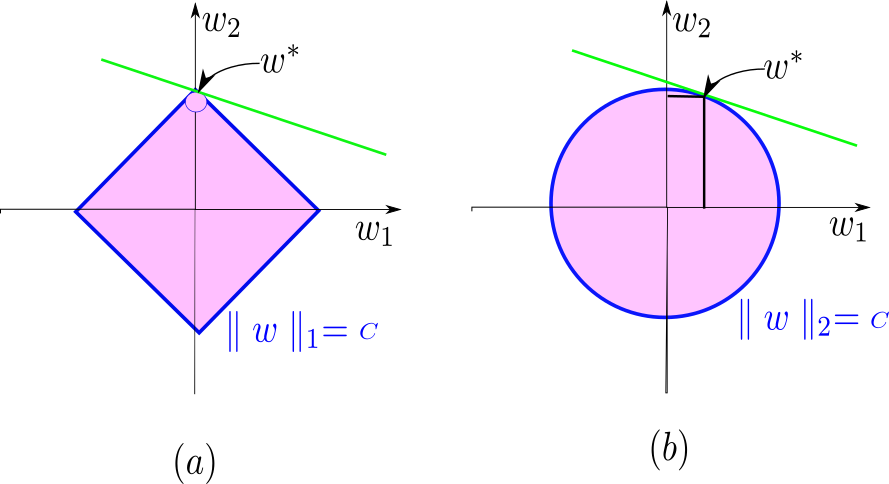
\includegraphics[width=4in]
{regularization/sparsity.png}
\caption{Pictorial explanation of
why $L^1$ norm ROLF can lead to sparsity
and $L^2$ norm ROLF can help avert it. Sometimes
you want sparsity and sometimes you don't. $c$ in this figure is some
fixed constant.
}
\label{fig-sparsity}
\end{figure}

Assume $\call(w)$ is linear in $w$.\footnote{What we say here about sparsity also applies in some cases when $\call(w)$ is not linear in $w$. For example, it applies sometimes when $\call(w)$
is quadratic in $w$ as occurs in Least Squares.}
For example,
\beq
\call(w)= Xw-y
\eeq
where $w\in\RR^n$, $X\in \RR^{nsam\times n}$,  and $y\in\RR^{nsam}$.
$nsam$ is often the number of samples. That's why we name it that way.
The set $A=\{w: Xw-y=c\}$ for some fixed constant $c$  might be empty,
or contain a single point or a line or a plane, or a hyperplane. Let $dof=n-nsam$
be the degrees  of freedom in $w$.
Barring some exceptional cases, if $dof\leq 0$, we expect $A$ to be empty.
If $dof=1$, we expect $A$ to trace out a line, if $dof= 2$, we expect $A$ to
trace out a plane, and so forth.

In Fig.\ref{fig-sparsity}, we imagine
what would happen if
$w\in \RR^2$, $X\in \RR^{1\times 2}$
and $y\in \RR$ so $A$ traces a line,
represented in green.
In Fig.\ref{fig-sparsity} $(a)$,
we imagine that $\calr(w)=\norm{w}_1$
and in Fig.\ref{fig-sparsity} $(b)$, that
$\calr(w)=\norm{w}_2^2$.
For points $w$ such that $\calr(w)$
has a well defined gradient,
minimization of
\beq
\call^+(w) = \call(w) +\calr(w)
\eeq
requires that the $w$-gradients of
$\call$ and $\calr$ be equal in magnitude but opposite in direction.

\beq
\nabla_w\call = -\nabla_w \calr
\eeq
But when $\calr(w)$ is
the $L^1$ norm,  $\nabla_w\calr$ is not defined along the $w_1$
and $w_2$ axes. To avoid this, we can
approximate the diamond contour $\norm{w}_1=c$
by rounding out its corners
by an infinitesimal amount. If the green line had
slope of $-1$,
there would be a diamond contour
 $\norm{w}_1=c$ that would coincide with the green line along the
 segment connecting points $(0,c)$
 and $(c,0)$. However, this is an exceptional case. Usually, the slope
 of the green line is not $\pm 1$.
 In that case, the only way for
 $\call$ and $\calr$ to have
 opposite gradients is if the diamond
 contour and the green line
 kiss at one of the (rounded)  corners
 of the diamond contour. Call that
 kissing point $w^*$. Note from
 Fig.\ref{fig-sparsity} $(a)$ that kissing point $w^*=(0,c)$ would be
 sparse. In going from the Fig.\ref{fig-sparsity} $(a)$ to Fig.\ref{fig-sparsity} $(b)$,
 we have replaced the diamond contour
 $\norm{w}_1=c$ by
 a circular contour $\norm{w}_2=c$,
 but we have kept the same green line.
 Note that with the circular contour,
 the kissing point $w^*$ is no longer sparse; both of its components are non-zero.

 The moral of Fig.\ref{fig-sparsity}
 is that $L^1$ norm ROLF can lead to sparsity and $L^2$ norm ROLF can help avert it.
 Sometimes we want the vector of weights $w$ to be sparse so as to give
 a succinct description.
 At other times, we want solutions in set $A$ to be spread out over many dimensions instead of being sparse and clumped together in a small number of dimensions.






\subsection{$L^2$ norm ROLF for Least Squares}
As in Chapter \ref{ch-linear-reg} on Linear Regression,
suppose $w\in\RR^n$, $X\in \RR^{nsam\times n}$,
 and  $y\in\RR^{nsam} $. Let

\beq
\call^+(w)=\call(w) + \calr(w)
\eeq
where

\beq
\call(w)=
\frac{1}{n}
(Xw-y)^T(Xw-y)
\eeq
and

\beq
\calr(w) =\lam\norm{w}^2_2
\;.
\eeq
If we vary the  vector $w$ by an
infinitesimal amount $\delta w^T$, we get

\beq
0= \delta\call^+(w)=
\delta w^T
\left[\frac{2X^T}{n}(Xw-y) +2 \lam w \right]
\eeq
Hence

\beq
X^T(Xw-y)+\lam n  w=0
\eeq

\beq
(X^TX+\lam n)w = X^T y
\eeq

\beqa
w&=&
(X^TX + \lam  nI)^{-1}X^Ty
\\
&=&
\frac{1}{\lam n}(I +
\frac{X^T X}{\lam n})^{-1}X^Ty
\eeqa

Note that for $\lam=0$, the minimum $w^*$ of $\call^+(w)$ is

\beq
w^*= (X^TX)^{-1}X^Ty
\;\;\text{(valid for $\lam=0$)}
\eeq
When $\lam>>1$,
we can express $w^*$  as a Taylor expansion in
$w$.
Recall that if $|\eps|<1$,
\beq
\frac{1}{1-\eps}=
1 + \eps + \eps^2 + \ldots
\eeq
Define
$n_0 = 1/\lam$,
and assume that
$\frac{n_0}{n}|X^TX| <1  $.
Then

\beqa
w^* &=& \frac{n_0}{n}
\sum_{i=0}^{\infty}
(-\;\frac{n_0 X^TX}{n})^i
X^Ty
\\
&=&
-\sum_{i=0}^{\infty}
\left(-\;\frac{n_0 X^TX}{n}\right)^{i+1}
(X^TX)^{-1}X^Ty
\;\;\text{(valid for $\lam=\frac{1}{n_0}>>1$)}
\eeqa
Truncating this series is itself
a kind of regularization.


\section{Proximal functions}

For $v \in \RR^n$, $w\in \WW \subset \RR^n$
and $\alp>0$, we define the
{\bf proximal function}
$w^{prox}:\RR^n \rarrow \WW$ by

\beq
\boxed{
w^{prox}(v; \alp\call, \WW) = \argmin_{w\in \WW}
\underbrace{
\left(
\call(w) +
\underbrace{ \frac{1}{2\alp}\norm{w-v}^2}_{\calr(w,v)}
\right)}_{\call^+(w, v)}}
\eeq
$w^{prox}(v)$ can be viewed as a
projection of $v\in\RR^n$
onto $w$ in the subspace $\WW\subset \RR^n$.
Henceforth we assume $\WW=\RR^n$,
so the projected vector $v$ and
its projection $w$ are in the same
vector space $\RR^n$.

See Fig.\ref{fig-proximal-example}
for a numerical example of a
proximal function $w^{prox}:\RR\rarrow \RR$.


\begin{figure}[h!]
\centering
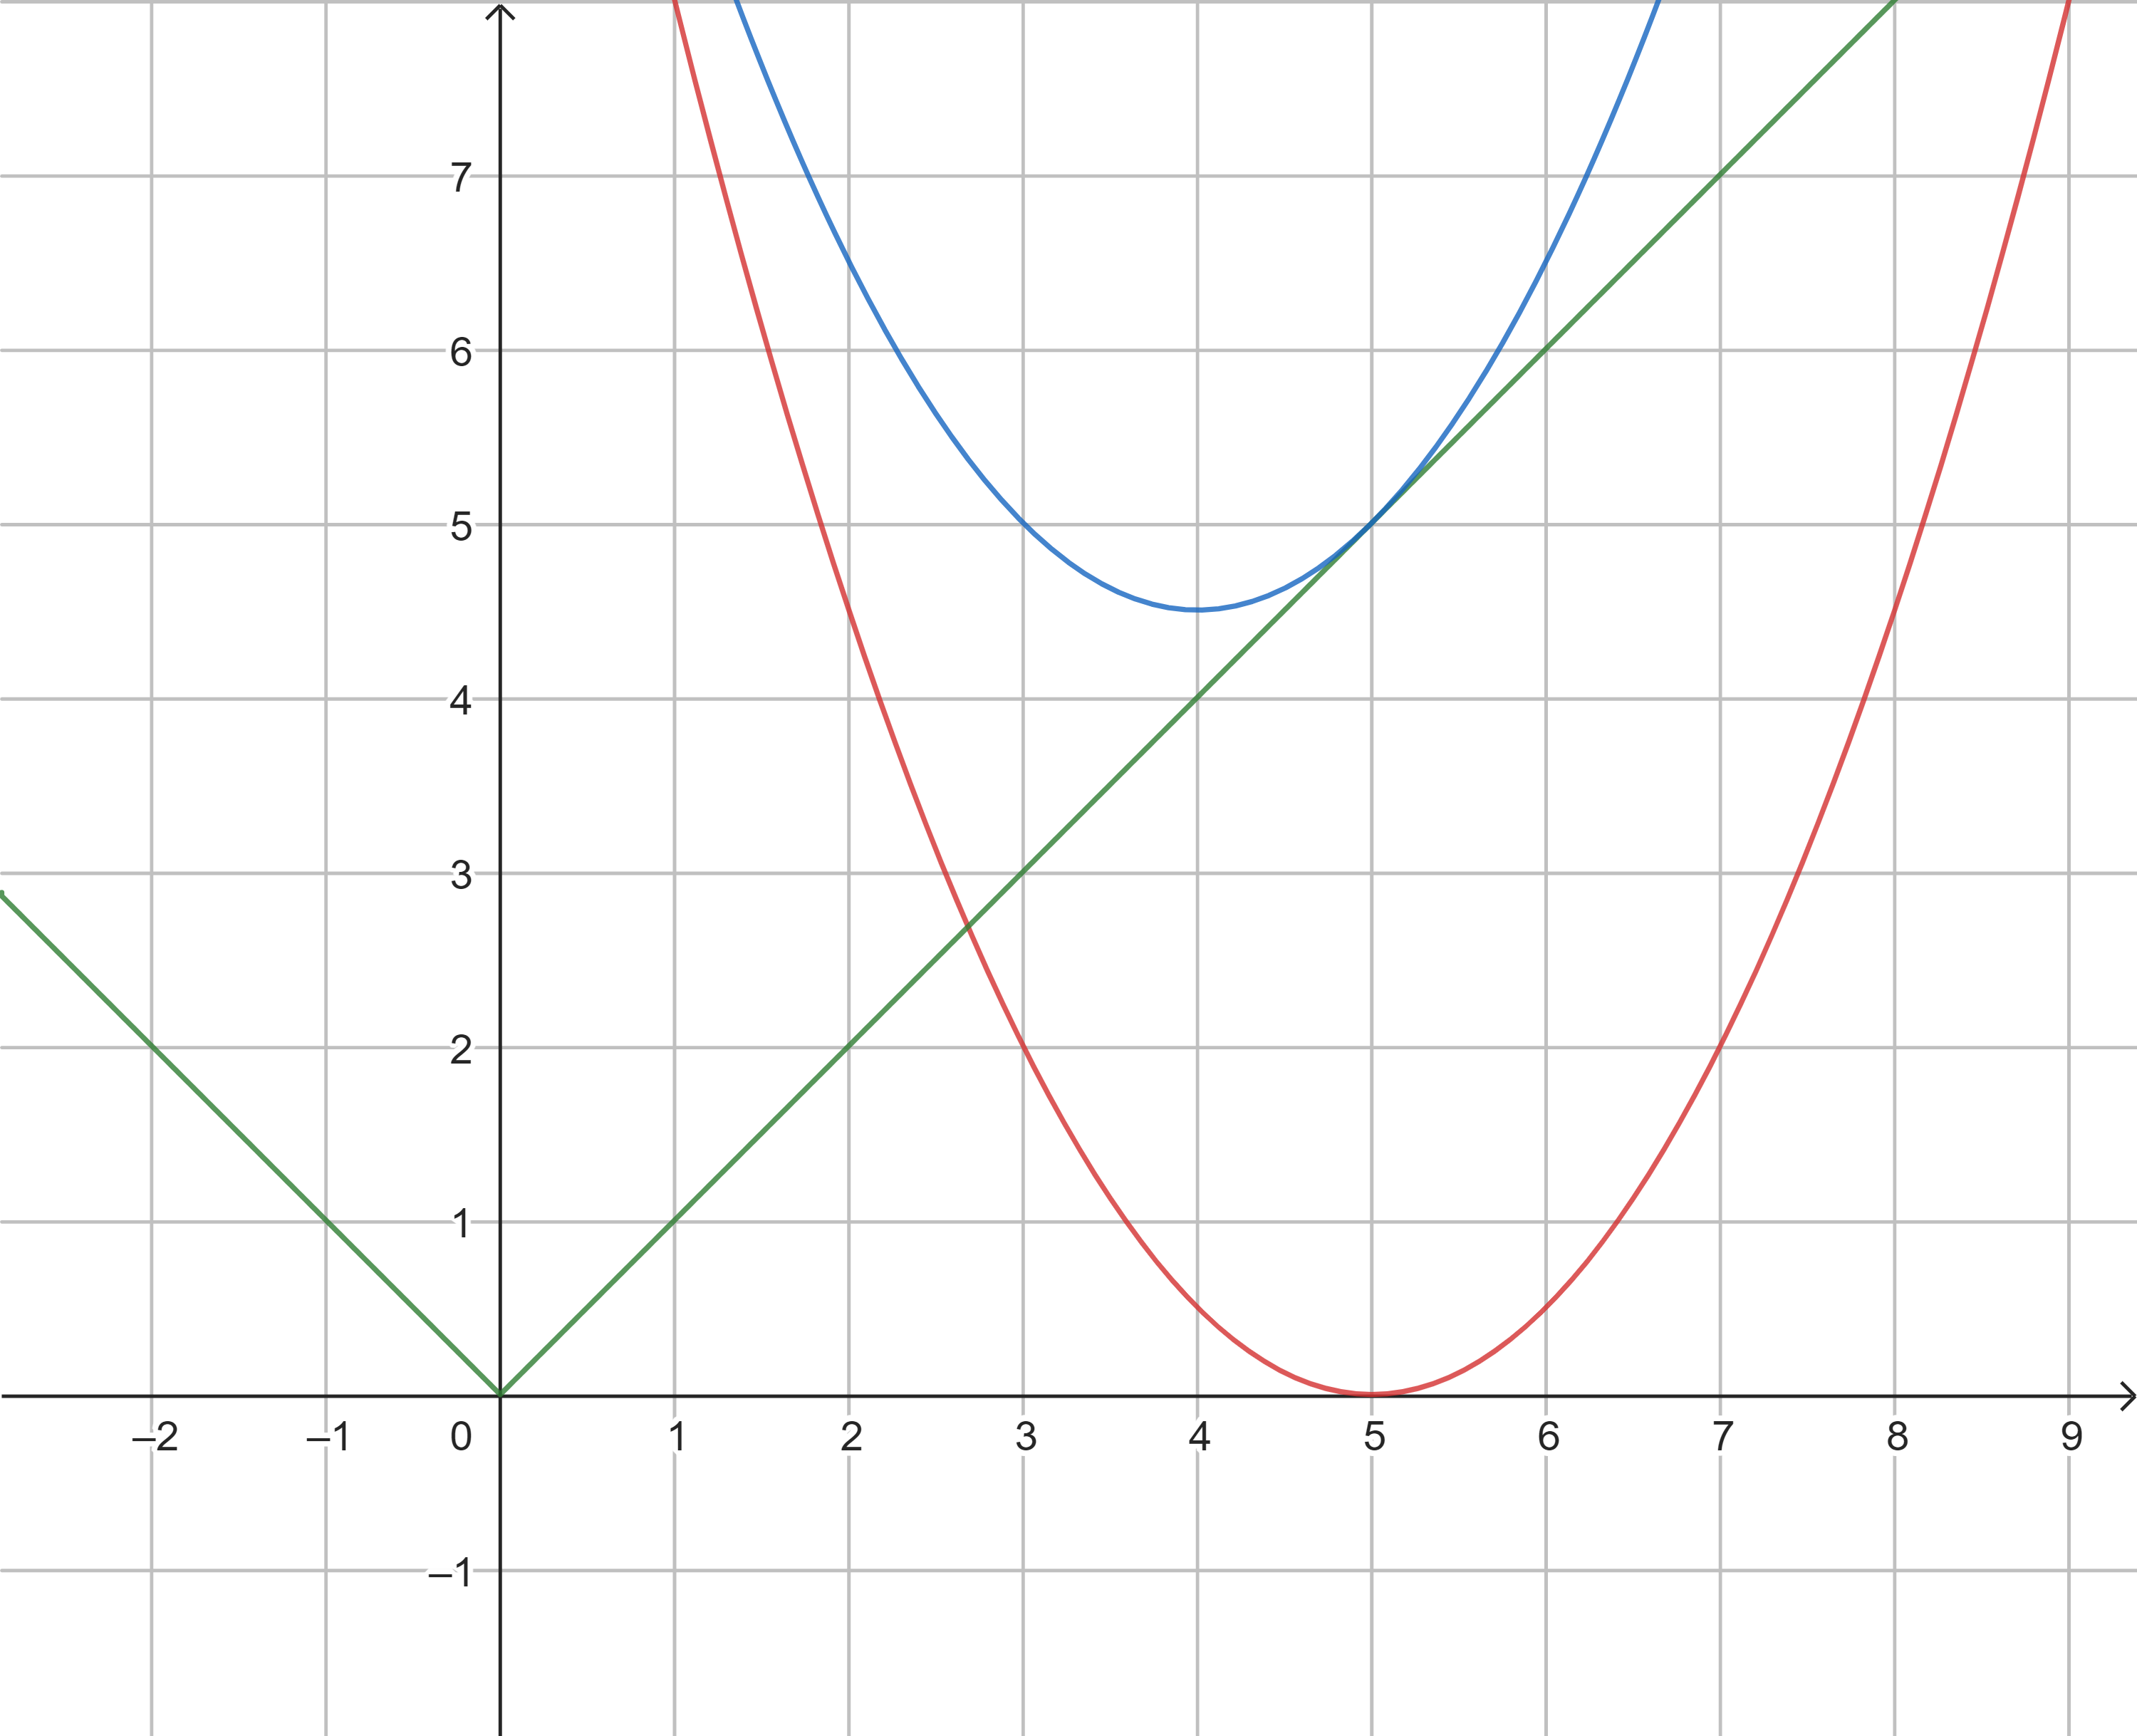
\includegraphics[width=3in]
{regularization/proximal-example.png}
\caption{Example of a proximal
function. x-axis is $w$ and $v=5$. Green curve: $\call(w)=|w|$. Red curve: $\calr(w, 5)=\frac{1}{2}(w-5)^2$, Blue curve: $\call^+(w, 5)=\call(w)+\calr(w,5)$. Note that we are adding 2 convex functions so the minimum of the sum is somewhere in between the minima of the two summands.
$w^{prox}(5) =\argmin_w
\call^+(w, 5)=4$.
}
\label{fig-proximal-example}
\end{figure}

Next, we will discuss an
analytical rather a numerical
example of proximal functions.
We  begin by defining the
shrinking function\footnote{We call it a
{\bf shrinking function} because
it shrinks a neighborhood-of-zero to zero.
Another common name for this function is a
 {\bf soft-threshold function}, because
 it makes the transition from negative to positive y axis values occur over the interval of $x\in [-\alp, \alp]$ instead of $x\in [0,0]$.}
 $sh_0: \RR\rarrow \RR$ and its inverse
$sh_0^{-1}:\RR\rarrow\RR$  for any $\alp>0$:

\beq
sh_0(v; \alp) = (v-\alp)\indi(v>\alp) + (v+\alp)\indi(v<-\alp)
\eeq

\beq
sh^{-1}_0(w; \alp) = (w+\alp)\indi(w>0) + (w-\alp)\indi(w<0)
\eeq
Fig.\ref{fig-sh_0_w}
shows a plot of $sh_0$ and
$sh^{-1}_0$.


\begin{figure}[h!]
\centering
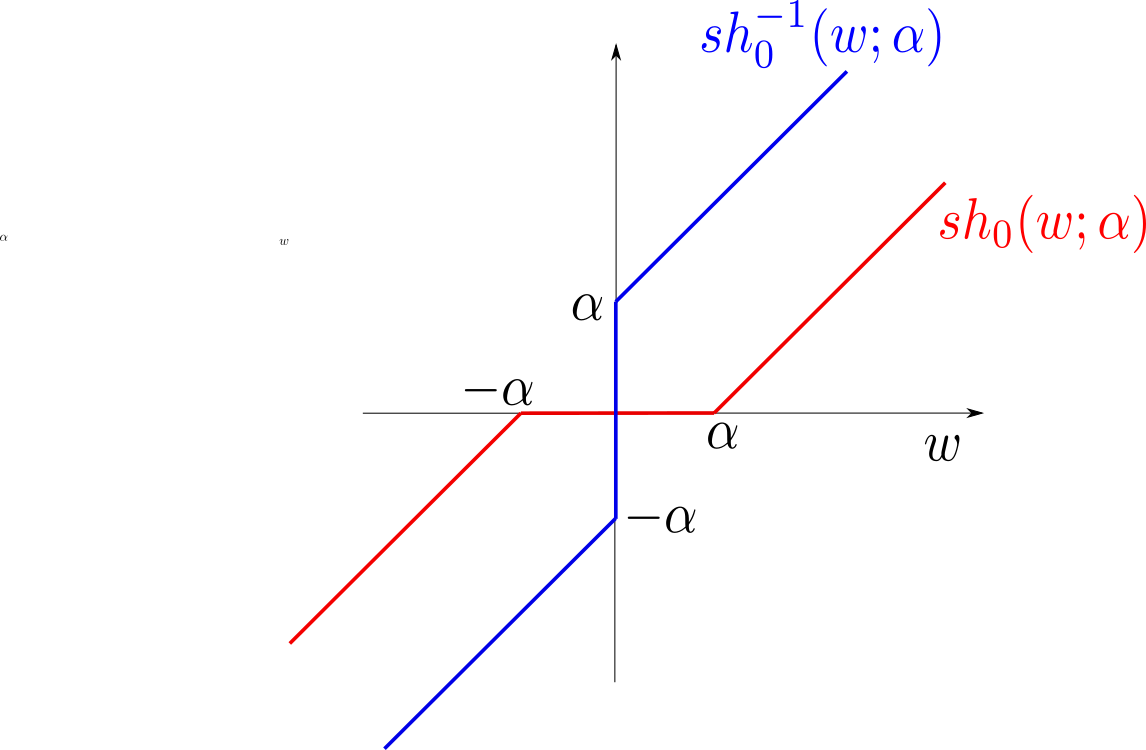
\includegraphics[width=3.7in]
{regularization/sh_0_w.png}
\caption{Plot
of the functions $sh_0(w; \alpha)$ and $sh_0^{-1}(w; \alpha)$.
}
\label{fig-sh_0_w}
\end{figure}

\begin{claim}
For $\WW=\RR$ and $w, v\in\RR$, if
\beq
\call(w)= |w|
\;,
\eeq
then

\beq
w^{prox}(v) = sh_0(v; \alp)
\eeq
and


\beq
\call^+(w^{prox}(v), v)
=
|sh_0(v; \alp)| + \frac{\alp}{2}
\eeq

\end{claim}
\proof
\beq
0=\frac{d\call^+}{dw}
=
\alp[\indi(w>0)-\indi(w<0)] + (w-v)
\eeq
So

\beqa
v &=& w+ \alp [\indi(w>0)-\indi(w<0)]
\\
&=& (w+\alp)\indi(w>0) + (w-\alp) \indi(w<0)
\\
&=& sh^{-1}_0(w; \alp)
\eeqa
Hence

\beq
w^{prox}(v;\alp) = sh_0(v; \alp)
\eeq

Note that

\beq
|w-v| = |\alp|
\eeq
so
\beqa
\call^+(w_{prox}(v), v)&=&|w^{prox}(v;\alp)|
+ \frac{\alp}{2}
\\
&=&
|sh_0(v; \alp)| + \frac{\alp}{2}
\eeqa
\qed




\section{Proximal ROLF}

Proximal functions can be
used to do ROLF as follows.
For $w,v\in\RR^n$
and $\alp>0$,  let

\beq
\calr(w, v) = \frac{1}{2\alp}\norm{w-v}^2_2
\eeq
and\footnote{Note
that $\call$ here could be the mean square error
plus an $L^p$ norm. A loss function plus a regulator function gives
a new loss function to
which a new regulator may be added.
}

\beq
\call^+(w) = \call(w) + \calr(w, w^*)
\;,
\eeq
where $w^*$ is the $w$-minimum
of both $\call(w)$ and $\calr(w, w^*)$:


\beq
w^* = \argmin_w \call(w)
=\argmin_w \calr(w, w^*)
\eeq
Hence,

\beq
w^* = \argmin_w \left[ \call(w) +
\calr(w, w^*)\right]
\;.
\eeq
Now assume the sequence of
points $\{w_k\}_{k=0}^\infty$
satisfies
$w_k \rarrow w^*$ as
 $k
\rarrow \infty$. Then

\beq
w_{k+1}=
\underbrace{\argmin_w
\left(\call(w) + \frac{1}{2\alp}
\norm{w-w_k}^2_2\right)
}_{w^{prox}(w_k)}
\eeq
If we differentiate
the argument of argmin()
to find its minimum, we find

\beq
0= \alp
\underbrace{\nabla_w\call(w_{k+1})}_{\approx \nabla_w\call(w_{k})}+ w_{k+1}-w_k
\eeq

Thus, the following 3 recursion relations\footnote{Some people use a sequence $\alp_k\in \RR_+$ instead of the constant $\alp>0$. This is called an
{\bf adaptive step size}
and can yield faster
convergence rates.}
can be used to calculate $w_k$:

\begin{subequations}

\beq
\boxed{
w_{k+1}  = w_{k} -\alp\nabla_w\call(w_{k})}
\xymatrix{
&&\ar[d]^{-\alp\nabla_w\call(w_k)}\\
\ar[rr]_{w_{k+1}}\ar[rru]^{w_k}&&
}
\label{eq-non-prox-steep-d}
\eeq


\beq
\boxed{
w_{k+1}=
w^{prox}(w_k)}
\eeq


\beq
\boxed{
w_{k+1}=
w^{prox}(w_k-\alp \nabla_w\call(w_k))}
\label{eq-prox-steep-d}
\eeq
\end{subequations}

Eq.(\ref{eq-non-prox-steep-d}) is the familiar
recursion relation for
gradient
descent (See Chapter \ref{ch-gradient-descent}).
Eq.(\ref{eq-prox-steep-d})
combines gradient descent
and a proximal projection,
so it is expected to
converge faster than
simple gradient descent.

\section{Unobserved Nodes of a bnet}

Nodes of a bnet for which the CPT is unknown are called unobseved nodes.
In this book, \hiddenNodes


{\bf Unobserved nodes} (UN) represent what are called
 {\bf latent random variables} in Statistics.

 UN make an appearance in many
 places throughout this book.
 For example, they are essential
 to the methods of
 Kalman Filtering (see Chapter \ref{ch-kalman}) and
 Hidden Markov Model (see Chapter \ref{ch-hmm}).

This being a book about bnets and a chapter about ROLF,
we would like to stress that UN
can be viewed as a very natural and powerful way of
doing (implicit) ROLF when using bnets.
